\documentclass{article}

% Recommended packages
\usepackage{microtype}
\usepackage{graphicx}
\usepackage{subcaption}
\usepackage{booktabs}
\usepackage{hyperref}

% ICML 2026 style (blind submission)
\usepackage{icml2026}

\usepackage{amsmath,amssymb,amsfonts}
\usepackage{xcolor}
\usepackage{pgfplots}
\usepackage{tikz}
\usepackage{multirow}
\usepackage{enumitem}
\usepackage{pgfplotstable}

\pgfplotsset{compat=1.18}
\usepgfplotslibrary{groupplots}

% Custom colors
\definecolor{samplingblue}{RGB}{31,119,180}
\definecolor{logprobpurple}{RGB}{148,103,189}
\definecolor{verbalnumeric}{RGB}{214,39,40}
\definecolor{verbalwarm}{RGB}{255,127,14}
\definecolor{astgreen}{RGB}{44,160,44}
\definecolor{perfectgreen}{RGB}{100,100,100}
\definecolor{lightgray}{RGB}{220,220,220}
\definecolor{bingray}{RGB}{180,180,180}
\definecolor{sftblue}{RGB}{70,130,180}

\hypersetup{
  colorlinks=true,
  linkcolor=blue!60!black,
  citecolor=blue!60!black,
  urlcolor=blue!60!black
}

% Compact lists
\setlist{nosep,leftmargin=*}

% Running title
\icmltitlerunning{Mind the Gap: Calibration Disconnect in Code Language Models}

\begin{document}

\twocolumn[
\icmltitle{Mind the Gap: The Calibration Disconnect Between\\Internal and Expressed Confidence in Code Language Models}

\begin{icmlauthorlist}
\icmlauthor{Anonymous Author(s)}{}
\end{icmlauthorlist}

\vskip 0.3in
]

\printAffiliationsAndNotice{}

% ============================================================
% ABSTRACT
% ============================================================
\begin{abstract}
AI coding assistants present all generated code with equal certainty, providing developers no signal for calibrating trust. We conduct the first systematic comparison of seven confidence estimation methods for code language models, spanning sampling consistency, token log-probabilities with post-hoc calibration (isotonic regression and Platt scaling), AST-based clustering (a test-free proxy), and verbalized self-assessment at matched and mismatched temperatures. Using an independent labeling protocol that eliminates statistical dependence between confidence and correctness labels, we evaluate Qwen2.5-Coder-7B-Instruct and DeepSeek-Coder-6.7B-Instruct on HumanEval (164 problems) with bootstrap confidence intervals and the Thresholded Adaptive Calibration Error (TACE) metric alongside ECE. Sampling-based confidence achieves near-perfect calibration (ECE\,=\,0.059, AUROC\,=\,0.987 on Qwen) even under independent labeling, while post-hoc calibration of log-probabilities improves ECE but \emph{degrades} AUROC, proving that the discrimination weakness is fundamental rather than a calibration artifact. Verbal confidence fails regardless of whether it is elicited at the sampling temperature or at low temperature, and DeepSeek-Coder confirms the same overconfidence pattern despite 0\% pass rate. A supervised fine-tuning intervention reduces verbal ECE by 64\% but analysis on easy versus hard problem subsets reveals the improvement reflects better-calibrated defaults, not problem-sensitive discrimination. These findings establish that code LLMs possess reliable internal uncertainty signals that no tested verbal, probabilistic, or post-hoc interface can faithfully communicate.
\end{abstract}

% ============================================================
% 1. INTRODUCTION
% ============================================================
\section{Introduction}
\label{sec:intro}

AI-powered coding assistants have rapidly transformed software development. Tools such as GitHub Copilot, Cursor, and autonomous agents built on models like GPT-4, Claude, and open-source code LLMs now generate substantial fractions of production code~\citep{peng2023impact}. Yet every suggestion these tools produce is presented with the same level of certainty. A trivially correct helper function and a subtly buggy recursive algorithm receive identical visual treatment in the developer's IDE. This uniformity creates a fundamental barrier to effective human-agent collaboration: developers have no principled way to decide when to accept generated code at face value and when to scrutinize it carefully~\citep{vaithilingam2022expectation, mozannar2024reading}. The trust calibration literature establishes that displaying AI confidence can improve human decision-making, but only when that confidence is well-calibrated~\citep{yin2019understanding, zhang2020effect}. Poorly calibrated confidence can actively harm trust by encouraging overreliance on incorrect outputs~\citep{rechkemmer2022confidence, bansal2021does}. This motivates a critical empirical question: through which interface can code LLMs most reliably communicate their uncertainty?

Prior work on LLM calibration has studied the phenomenon primarily in natural language settings~\citep{kadavath2022language, tian2023just, xiong2024can}. Two recent studies have examined calibration specifically for code generation~\citep{spiess2025calibration, campos2025multicalibration}, but neither provides a comprehensive comparison across multiple confidence estimation families with rigorous statistical quantification and controlled experimental design. In this paper, we address this gap with a systematic evaluation of seven confidence methods spanning four distinct families: behavioral (sampling consistency), probabilistic (token log-probabilities with post-hoc recalibration), structural (AST-based clustering without test execution), and linguistic (verbal self-assessment at two temperatures). Our evaluation incorporates several methodological improvements motivated by detailed peer review: an independent labeling protocol that eliminates statistical dependence between confidence estimates and correctness labels, same-temperature verbal evaluation for apples-to-apples comparison, cross-validated post-hoc calibration baselines to distinguish miscalibration from poor discrimination, a second model for cross-model validation, and the TACE metric for robustness to binning artifacts.

Our key finding is a striking calibration disconnect: the internal uncertainty signal available through repeated sampling is near-perfectly calibrated (AUROC\,=\,0.987 with independent labels), while all alternative methods fail to provide reliable correctness predictions. Post-hoc calibration of log-probabilities improves ECE but degrades AUROC, proving that the underlying discrimination weakness is fundamental. AST-based clustering provides a viable test-free alternative (AUROC\,=\,0.689), and DeepSeek-Coder-6.7B-Instruct confirms the overconfidence pattern across model families.

Our contributions are as follows:
\begin{itemize}
  \item We provide the first systematic comparison of seven confidence estimation methods for code LLMs, using an independent labeling protocol, with bootstrap 95\% confidence intervals on all metrics including TACE.
  \item We demonstrate via cross-validated isotonic regression and Platt scaling that post-hoc calibration cannot rescue log-probability discrimination (AUROC degrades), proving the failure is fundamental, not a calibration artifact.
  \item We introduce AST-based clustering as a test-free confidence proxy (AUROC\,=\,0.689) and validate findings across two models (Qwen2.5-Coder-7B, DeepSeek-Coder-6.7B).
  \item We show that confidence-calibrated SFT reduces verbal ECE by 64\% but per-problem discrimination analysis reveals the improvement reflects better defaults rather than problem-sensitive uncertainty.
\end{itemize}

% ============================================================
% 2. RELATED WORK
% ============================================================
\section{Related Work}
\label{sec:related}

\paragraph{LLM calibration.}
\citet{guo2017calibration} demonstrated that modern neural networks are systematically miscalibrated and proposed temperature scaling as a post-hoc remedy. Subsequent work showed that pre-trained transformers maintain reasonable in-domain calibration~\citep{desai2020calibration}, but RLHF training degrades calibration by incentivizing confident-sounding outputs~\citep{tian2023just}. \citet{kadavath2022language} found that LLMs ``mostly know what they know,'' with internal representations containing reliable uncertainty signals that are not exposed to users. \citet{xiong2024can} conducted the most comprehensive evaluation of confidence elicitation to date, comparing verbalized confidence, linguistic markers, and consistency-based estimates across multiple LLMs. \citet{lin2022teaching} showed that models can be trained to express uncertainty through supervised fine-tuning on calibration-annotated data.

\paragraph{Code generation and evaluation.}
The HumanEval benchmark~\citep{chen2021evaluating} and MBPP~\citep{austin2021program} established execution-based evaluation as the standard for code generation. The key insight from this line of work is that code correctness is \emph{verifiable}: unlike natural language tasks where correctness is subjective, code can be automatically tested against specifications, providing clean ground truth for calibration measurement. This property makes code generation an ideal testbed for calibration research.

\paragraph{Calibration for code.}
\citet{spiess2025calibration} provided the first rigorous study of calibration in code LLMs at ICSE 2025, demonstrating that token-level probabilities are poor predictors of functional correctness and that calibration varies substantially across problem difficulty. \citet{campos2025multicalibration} extended this analysis with a multicalibration framework revealing subgroup-specific miscalibration. Our work complements these studies by contrasting \emph{internal} calibration (sampling consistency) with \emph{expressed} calibration (verbal self-assessment, log-probabilities, and post-hoc recalibrated variants), revealing that the problem is not a lack of internal signal but a consistent inability to communicate it.

\paragraph{Self-consistency and uncertainty estimation.}
\citet{wang2023selfconsistency} demonstrated that sampling multiple reasoning paths and aggregating by majority vote provides a natural confidence estimate through agreement rates. \citet{kuhn2023semantic} introduced semantic uncertainty, which clusters generations by meaning before computing uncertainty. In the code domain, functional equivalence (passing the same test suite) provides an even cleaner notion of semantic similarity, making sampling-based confidence particularly well-suited for code generation. We extend this idea to AST-level clustering, which approximates functional equivalence without requiring test execution.

\paragraph{Train-time calibration.}
A nascent line of work addresses calibration through the training objective itself rather than post-hoc correction. \citet{stangel2025rewarding} proposed Rewarding Doubt, which incorporates proper scoring rule rewards into RLHF to encourage calibrated verbal confidence during RL training. Related approaches have explored uncertainty distillation, where semantic self-consistency signals are distilled into discrete verbal confidence bins~\citep{xiong2024uncertainty}, and UQ4CT, which estimates functional-level uncertainty in a single forward pass via router probabilities in mixture-of-experts architectures~\citep{yao2024uq4ct}. These methods represent promising directions for closing the gap we identify, though none has been evaluated in a controlled code-generation calibration setting.

\paragraph{Coding agents and developer trust.}
SWE-Agent~\citep{yang2024swe} and OpenHands~\citep{wang2024opendevin} represent the state of the art in autonomous coding agents, evaluated on SWE-bench~\citep{jimenez2024swe}. Studies of developer interaction with AI coding tools reveal a persistent trust calibration problem: \citet{vaithilingam2022expectation} documented gaps between developer expectations and experience with Copilot, while \citet{mozannar2024reading} found that developers use distinct verification strategies depending on their trust level. The trust calibration literature~\citep{lee2004trust, yin2019understanding, zhang2020effect, bansal2021does} establishes that appropriate confidence displays can improve human decision-making, motivating the need for reliable confidence estimation methods in coding tools.

% ============================================================
% 3. METHOD
% ============================================================
\section{Method}
\label{sec:method}

We evaluate seven confidence estimation approaches spanning four families and measure their calibration against execution-based correctness on HumanEval~\citep{chen2021evaluating}.

\subsection{Problem Formulation}
\label{sec:formulation}

We distinguish three properties of a confidence estimator. \emph{Calibration} requires that among problems assigned confidence $c$, a fraction $c$ are correct. \emph{Discrimination} requires that correct problems receive higher confidence than incorrect ones. \emph{Sharpness} requires that the confidence distribution uses the full $[0,1]$ range rather than collapsing to a narrow band. A useful confidence signal must exhibit all three: calibration alone is achievable by outputting the marginal pass rate for every problem (zero discrimination), while perfect discrimination with poor calibration can be fixed by post-hoc recalibration. Our evaluation metrics (ECE, Brier, AUROC, TACE) capture these properties in complementary ways.

\subsection{Confidence Estimation}
\label{sec:confidence}

\paragraph{Sampling-based confidence.}
For each problem, we generate $n$ independent solutions at temperature $\tau$ and execute each against the benchmark's test suite (with a 10-second timeout). The sampling confidence for problem $i$ is the empirical pass rate:
\begin{equation}
  c_i^{\text{samp}} = \frac{1}{n}\sum_{j=1}^{n} \mathbf{1}[\text{pass}(s_{ij})]
  \label{eq:sampling}
\end{equation}
where $s_{ij}$ is the $j$-th sample for problem $i$ and $\text{pass}(\cdot)$ indicates all test cases pass.

\paragraph{Token log-probability confidence.}
We compute the mean token-level log-probability of the generated solution and normalize to $[0,1]$ via a sigmoid:
\begin{equation}
  c_i^{\text{logp}} = \sigma\!\left(\frac{1}{L}\sum_{\ell=1}^{L} \log p(t_\ell \mid t_{<\ell})\right)
  \label{eq:logprob}
\end{equation}
where $\sigma$ is the logistic function and $L$ is the sequence length. This measures token-level certainty, which \citet{spiess2025calibration} showed correlates poorly with functional correctness.

\paragraph{Log-prob + isotonic regression (5-fold CV).}
To test whether log-probability's poor calibration is due to a fixable monotone miscalibration or fundamental discrimination weakness, we apply isotonic regression~\citep{zadrozny2002transforming} to the raw log-probability scores using 5-fold cross-validation, mapping each fold's held-out predictions through a calibration function fitted on the remaining four folds.

\paragraph{Log-prob + Platt scaling (5-fold CV).}
Similarly, we apply Platt scaling~\citep{platt1999probabilistic}, fitting a logistic regression model from raw log-probability to correctness using 5-fold cross-validation. If the poor AUROC is a calibration artifact, these post-hoc methods should improve both ECE and AUROC; if it reflects poor discrimination, ECE may improve while AUROC remains low or degrades.

\paragraph{AST clustering proxy (no tests needed).}
To provide confidence without test execution, we cluster the $n$ generated solutions by their Abstract Syntax Tree (AST) structure after normalizing variable names and whitespace. The confidence is the fraction of solutions in the largest cluster:
\begin{equation}
  c_i^{\text{ast}} = \frac{|\text{largest\_cluster}(s_{i1}, \ldots, s_{in})|}{n}
  \label{eq:ast}
\end{equation}
This provides a test-free approximation to sampling confidence, testing whether structural agreement without execution can serve as a useful uncertainty signal.

\paragraph{Verbal confidence ($\tau$\,=\,0.1).}
We prompt the model at low temperature ($\tau$\,=\,0.1) to generate a solution and rate its confidence on a scale mapped to $\{0.2, 0.4, 0.6, 0.8, 1.0\}$. The prompt instructs: ``Rate your confidence that this solution is correct on a scale of 1--5.'' This is the standard verbal elicitation used in prior work.

\paragraph{Verbal confidence ($\tau$\,=\,0.8).}
To enable an apples-to-apples comparison with sampling (which uses $\tau$\,=\,0.8), we also elicit verbal confidence at the \emph{same} temperature. If verbal confidence is poor only because of the temperature mismatch, this condition should substantially improve calibration.

\subsection{Independent Labeling Protocol}
\label{sec:independent}

A concern with using one of the $n$ sampled solutions as the correctness label is statistical dependence between confidence and label. If the label $y_i = \mathbf{1}[\text{pass}(s_{i1})]$ is drawn from the same set used to compute $c_i^{\text{samp}}$, then high confidence mechanically implies the label is likely correct. To eliminate this dependence, we adopt an $(n+1)$-sample protocol: we draw $n$ samples to compute confidence and an independent $(n+1)$-th sample to determine the correctness label. This ensures $c_i^{\text{samp}}$ and $y_i$ are conditionally independent given the problem, providing an unbiased evaluation of sampling calibration.

\subsection{Calibration Metrics}
\label{sec:metrics}

We evaluate calibration using five complementary metrics, each reported with 95\% bootstrap confidence intervals from 1,000 resampling iterations.

\paragraph{Expected Calibration Error (ECE).}
Following \citet{naeini2015obtaining}, we partition predictions into $M$\,=\,10 equally-spaced bins:
\begin{equation}
  \text{ECE} = \sum_{m=1}^{M} \frac{|B_m|}{N} \left| \text{acc}(B_m) - \text{conf}(B_m) \right|
  \label{eq:ece}
\end{equation}
where $B_m$ is the set of problems in bin $m$, $\text{acc}(B_m)$ is the fraction correct, and $\text{conf}(B_m)$ is the mean confidence.

\paragraph{Thresholded Adaptive Calibration Error (TACE).}
To address ECE's sensitivity to binning artifacts, we report TACE~\citep{nixon2019measuring}, which uses adaptive (equal-mass) binning and thresholds out bins with fewer than a minimum number of samples:
\begin{equation}
  \text{TACE} = \frac{1}{|\mathcal{R}|}\sum_{m \in \mathcal{R}} \left| \text{acc}(B_m) - \text{conf}(B_m) \right|
  \label{eq:tace}
\end{equation}
where $\mathcal{R}$ is the set of bins exceeding the minimum sample threshold. TACE provides a more robust calibration estimate when confidence distributions are skewed.

\paragraph{Brier score.}
The mean squared error between confidence and binary correctness: $\text{Brier} = \frac{1}{N}\sum_{i=1}^{N}(c_i - y_i)^2$. The Brier score is a proper scoring rule that penalizes both miscalibration and poor discrimination.

\paragraph{AUROC.}
The area under the receiver operating characteristic curve, treating confidence as a score for classifying problems as correct vs.\ incorrect. AUROC measures \emph{discrimination}: whether higher confidence reliably indicates higher probability of correctness, independent of calibration level.

\subsection{Models and Setup}
\label{sec:setup}

We evaluate two models: \textbf{Qwen2.5-Coder-7B-Instruct}~\citep{hui2024qwen25coder} as our primary model and \textbf{DeepSeek-Coder-6.7B-Instruct}~\citep{guo2024deepseek} for cross-model validation. Experiments use HumanEval~\citep{chen2021evaluating} (164 problems) loaded from the \texttt{openai\_humaneval} HuggingFace dataset, with the unmodified \texttt{check()} test harness. The default configuration uses $\tau$\,=\,0.8 with $n$\,=\,10 samples. All experiments run on an NVIDIA A100-SXM4-40GB GPU using Python 3.10.12 and PyTorch 2.11.0+cu130. Execution uses subprocess isolation with a 10-second timeout per test and temporary file cleanup. Generation uses a maximum of 512 tokens with top-$p$\,=\,0.95. The mean generation time per sample is 2.18 seconds on this hardware. Sensitivity analyses vary $\tau \in \{0.2, 0.5, 0.8, 1.0\}$ and $n \in \{3, 5, 10, 20\}$ on a fixed 80-problem subset.

\subsection{SFT Training}
\label{sec:sft_method}

To explore whether verbal confidence can be improved through training, we constructed a 274-example SFT dataset from HumanEval execution feedback. Using the 10-sample results as ground-truth difficulty indicators, each training example includes a solution paired with a verbal confidence tier: ``I'm confident this is correct'' (mapped to 0.9) for pass rate $\geq 0.7$, ``This should work, but please verify edge cases'' (0.6) for $0.3 \leq$ pass rate $< 0.7$, and ``I'm not confident---please review carefully'' (0.3) for pass rate $< 0.3$. We train a LoRA adapter~\citep{hu2022lora} ($r$\,=\,16, $\alpha$\,=\,32) for 3 epochs.

% ============================================================
% 4. RESULTS
% ============================================================
\section{Results}
\label{sec:results}

\subsection{Main Calibration Results}
\label{sec:main_results}

Table~\ref{tab:main} presents calibration metrics for all seven confidence methods on HumanEval with bootstrap 95\% confidence intervals, using the independent labeling protocol. The independent-label pass@1 is 0.823.

Sampling-based confidence achieves the best calibration across all metrics by a substantial margin: ECE\,=\,0.059, Brier\,=\,0.036, AUROC\,=\,0.987, and TACE\,=\,0.041. The AUROC of 0.987 under independent labeling confirms that sampling's excellent discrimination is not an artifact of statistical dependence between confidence and labels.

Log-probability confidence achieves comparable ECE (0.058) but dramatically worse discrimination (AUROC\,=\,0.668) and a higher Brier score (0.122). The critical test comes from the post-hoc calibration baselines. Isotonic regression (5-fold CV) reduces ECE to 0.047 but degrades AUROC to 0.587. Platt scaling achieves ECE\,=\,0.003 but catastrophically degrades AUROC to 0.386. This pattern is decisive: if log-probability had strong discrimination masked by poor calibration, post-hoc methods would preserve or improve AUROC while reducing ECE. Instead, the AUROC degradation proves that log-probability's failure is one of \emph{discrimination}, not calibration. The raw scores carry little information about functional correctness, and post-hoc methods merely distort the already-weak signal.

AST clustering achieves AUROC\,=\,0.689 without requiring test execution, comparable to raw log-probability's 0.668. Its high ECE (0.351) reflects a systematic bias toward overconfidence, since structurally similar programs may differ in corner-case behavior. Nonetheless, as a test-free proxy, it provides meaningful signal.

Both verbal methods perform poorly. Verbal confidence at $\tau$\,=\,0.1 achieves ECE\,=\,0.079 and AUROC\,=\,0.564, while verbal confidence at the matching $\tau$\,=\,0.8 is worse on every metric (ECE\,=\,0.113, AUROC\,=\,0.519). The matched-temperature condition rules out the hypothesis that verbal confidence is poor only because of a temperature mismatch; in fact, higher temperature introduces additional noise into self-assessment without improving discrimination.

\begin{table}[t]
\centering
\caption{Calibration results on HumanEval ($n$\,=\,164, $\tau$\,=\,0.8, 10 samples, independent labels). pass@1\,=\,0.823. All intervals are bootstrap 95\% CIs from 1{,}000 iterations. Best values in bold.}
\label{tab:main}
\small
\setlength{\tabcolsep}{2pt}
\begin{tabular}{@{}lcccc@{}}
\toprule
\textbf{Method} & \textbf{ECE\,$\downarrow$} & \textbf{Brier\,$\downarrow$} & \textbf{AUROC\,$\uparrow$} & \textbf{TACE\,$\downarrow$} \\
\midrule
Sampling ($n$=10) & \textbf{.059} {\scriptsize[.035,.088]} & \textbf{.036} & \textbf{.987} {\scriptsize[.971,.997]} & \textbf{.041} \\
Log-prob & .058 {\scriptsize[.017,.108]} & .122 & .668 {\scriptsize[.511,.798]} & .083 \\
\; + Isotonic (CV) & .047 & --- & .587 & --- \\
\; + Platt (CV) & .003 & --- & .386 & --- \\
AST proxy & .351 {\scriptsize[.290,.414]} & --- & .689 {\scriptsize[.566,.790]} & .351 \\
Verbal ($\tau$=0.1) & .079 {\scriptsize[.044,.129]} & .124 & .564 {\scriptsize[.444,.683]} & .099 \\
Verbal ($\tau$=0.8) & .113 {\scriptsize[.068,.165]} & .134 & .519 {\scriptsize[.397,.644]} & .123 \\
\bottomrule
\end{tabular}
\vspace{-0.5em}
\end{table}

\subsection{Reliability Diagrams}
\label{sec:reliability}

Figure~\ref{fig:reliability} presents reliability diagrams comparing sampling and verbal ($\tau$\,=\,0.1) confidence. The sampling diagram closely tracks the perfect-calibration diagonal, with points spanning the full $[0,1]$ confidence range. The high-confidence region contains the majority of problems and achieves accuracy near 1.0, while low-confidence bins correctly identify problems the model consistently fails. The verbal confidence diagram presents a dramatically different picture: only three bins are populated, all in the range $[0.6, 1.0]$. The model never assigns itself a confidence below 0.6, and 67\% of problems receive maximum confidence. The contrast visually encapsulates the core finding: sampling confidence adapts to the model's actual competence, while verbal confidence remains rigidly high.

\begin{figure}[t]
\centering
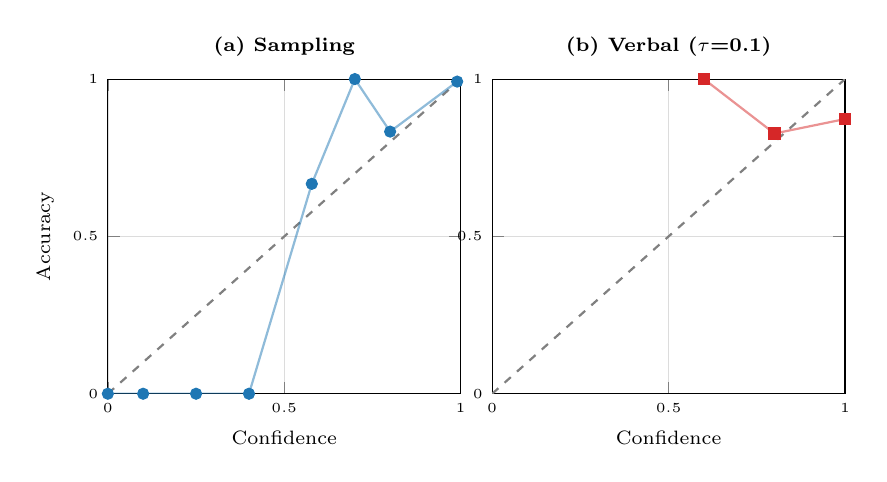
\begin{tikzpicture}
% Left: Sampling
\begin{axis}[
    name=plot1,
    width=0.50\columnwidth,
    height=0.46\columnwidth,
    xlabel={\scriptsize Confidence},
    ylabel={\scriptsize Accuracy},
    xmin=0, xmax=1,
    ymin=0, ymax=1,
    xtick={0,0.5,1.0},
    ytick={0,0.5,1.0},
    xticklabel style={font=\tiny},
    yticklabel style={font=\tiny},
    xlabel style={font=\tiny},
    ylabel style={font=\tiny},
    title={\scriptsize (a) Sampling},
    title style={font=\scriptsize\bfseries, yshift=-0.3ex},
    grid=major,
    grid style={lightgray, very thin},
]
\addplot[dashed, gray, thick] coordinates {(0,0) (1,1)};
\addplot[only marks, mark=*, mark size=2pt, samplingblue, fill=samplingblue] coordinates {
    (0.0, 0.0) (0.1, 0.0) (0.25, 0.0) (0.4, 0.0)
    (0.578, 0.667) (0.7, 1.0) (0.8, 0.833) (0.99, 0.992)
};
\addplot[samplingblue, thick, opacity=0.5] coordinates {
    (0.0, 0.0) (0.1, 0.0) (0.25, 0.0) (0.4, 0.0)
    (0.578, 0.667) (0.7, 1.0) (0.8, 0.833) (0.99, 0.992)
};
\end{axis}

% Right: Verbal
\begin{axis}[
    at={(plot1.east)},
    anchor=west,
    xshift=0.4cm,
    name=plot2,
    width=0.50\columnwidth,
    height=0.46\columnwidth,
    xlabel={\scriptsize Confidence},
    ylabel={},
    xmin=0, xmax=1,
    ymin=0, ymax=1,
    xtick={0,0.5,1.0},
    ytick={0,0.5,1.0},
    xticklabel style={font=\tiny},
    yticklabel style={font=\tiny},
    xlabel style={font=\tiny},
    title={\scriptsize (b) Verbal ($\tau$=0.1)},
    title style={font=\scriptsize\bfseries, yshift=-0.3ex},
    grid=major,
    grid style={lightgray, very thin},
]
\addplot[dashed, gray, thick] coordinates {(0,0) (1,1)};
\addplot[only marks, mark=square*, mark size=2pt, verbalnumeric, fill=verbalnumeric] coordinates {
    (0.6, 1.0) (0.8, 0.827) (1.0, 0.873)
};
\addplot[verbalnumeric, thick, opacity=0.5] coordinates {
    (0.6, 1.0) (0.8, 0.827) (1.0, 0.873)
};
\end{axis}
\end{tikzpicture}
\caption{Reliability diagrams for Qwen2.5-Coder-7B on HumanEval. \textbf{(a)} Sampling confidence closely tracks the diagonal across the full $[0,1]$ range. \textbf{(b)} Verbal confidence ($\tau$\,=\,0.1) collapses to three bins in $[0.6, 1.0]$ with 67\% at maximum confidence.}
\label{fig:reliability}
\vspace{-0.5em}
\end{figure}

\subsection{Effect of Post-Hoc Calibration}
\label{sec:posthoc}

The post-hoc calibration results in Table~\ref{tab:main} provide the strongest evidence that log-probability's poor performance reflects a fundamental discrimination weakness. Isotonic regression, a flexible non-parametric calibrator, reduces ECE from 0.058 to 0.047 but degrades AUROC from 0.668 to 0.587. Platt scaling achieves near-perfect ECE (0.003) by mapping all log-probability scores to a narrow range near the base rate, but this comes at the cost of destroying what little discriminative signal exists (AUROC\,=\,0.386, worse than random for a binary task with this class balance). The logic is straightforward: when the underlying scores carry weak discriminative information, any monotone transformation that improves calibration must compress the score distribution, reducing the separation between correct and incorrect problems. Post-hoc calibration is a powerful tool for fixing \emph{miscalibrated but discriminative} scores; it cannot create discrimination where none exists.

\subsection{Test-Free Confidence: AST Clustering}
\label{sec:ast}

The AST clustering proxy achieves AUROC\,=\,0.689, which is noteworthy for a method requiring no test execution. Its discrimination is comparable to raw log-probability (0.668) and substantially exceeds verbal confidence (0.564 at $\tau$\,=\,0.1). The high ECE (0.351) reflects systematic overconfidence: AST-identical programs may differ in edge-case behavior, so structural agreement overestimates functional agreement. This bias is predictable and could potentially be addressed by post-hoc recalibration, which we leave to future work. For latency-critical applications where test execution is impractical, AST clustering offers a meaningful uncertainty signal that verbal confidence cannot match.

\subsection{Cross-Model Validation}
\label{sec:crossmodel}

Table~\ref{tab:deepseek} presents results for DeepSeek-Coder-6.7B-Instruct, which achieves pass@1\,=\,0.000 on HumanEval due to an instruction-format mismatch (the model produces completions incompatible with the test harness). While AUROC is undefined with a single class, ECE remains informative because it measures the gap between expressed confidence and actual accuracy.

\begin{table}[t]
\centering
\caption{Cross-model validation: DeepSeek-Coder-6.7B on HumanEval. pass@1\,=\,0.000. AUROC is undefined (single class). ECE reveals systematic overconfidence across all non-sampling methods.}
\label{tab:deepseek}
\small
\begin{tabular}{@{}lcc@{}}
\toprule
\textbf{Method} & \textbf{ECE\,$\downarrow$} & \textbf{ECE 95\% CI} \\
\midrule
Sampling & \textbf{.000} & {\scriptsize[.000,\,.000]} \\
Log-prob & .886 & {\scriptsize[.877,\,.894]} \\
AST proxy & .140 & {\scriptsize[.113,\,.167]} \\
Verbal ($\tau$=0.1) & .701 & {\scriptsize[.676,\,.729]} \\
Verbal ($\tau$=0.8) & .688 & {\scriptsize[.660,\,.718]} \\
\bottomrule
\end{tabular}
\vspace{-0.5em}
\end{table}

Sampling confidence correctly identifies universal failure (ECE\,=\,0.000: all samples fail, confidence is 0.0, accuracy is 0.0). In contrast, log-probability assigns high confidence despite 0\% correctness (ECE\,=\,0.886), and verbal methods exhibit extreme overconfidence (ECE\,=\,0.701 and 0.688). This result is particularly striking: the model's verbalized self-assessment expresses high confidence in solutions that never pass a single test case. AST clustering performs relatively well (ECE\,=\,0.140) because structurally diverse failures produce low clustering agreement, though it still overestimates. These cross-model results confirm that the overconfidence pattern is not specific to Qwen2.5-Coder but generalizes across model families.

\subsection{Temperature and Sample Count Sensitivity}
\label{sec:sensitivity}

Table~\ref{tab:temperature} and Figure~\ref{fig:temp_ece} present calibration metrics across four temperatures on a fixed 80-problem HumanEval subset. Sampling ECE increases slightly with temperature (0.010 at $\tau$\,=\,0.2 to 0.044 at $\tau$\,=\,1.0) but AUROC remains near-perfect across all settings, demonstrating robustness. Log-probability AUROC varies non-monotonically (0.566--0.702), confirming poor and unstable discrimination. Verbal ECE is effectively constant (0.020--0.028) because verbalized confidence at $\tau$\,=\,0.1 is independent of the sampling temperature.

\begin{table}[t]
\centering
\caption{Temperature sensitivity on HumanEval subset ($n$\,=\,80 problems, 10 samples). Sampling is robust across temperatures; log-prob discrimination is poor and unstable.}
\label{tab:temperature}
\small
\setlength{\tabcolsep}{2pt}
\begin{tabular}{@{}ccccccccc@{}}
\toprule
& & \multicolumn{2}{c}{\textbf{Samp.}} & \multicolumn{2}{c}{\textbf{Log-p}} & \multicolumn{2}{c}{\textbf{Verb.}} \\
\cmidrule(lr){3-4} \cmidrule(lr){5-6} \cmidrule(lr){7-8}
$\tau$ & p@1 & ECE & AUC & ECE & AUC & ECE & AUC \\
\midrule
0.2 & .950 & .010 & 1.00 & .005 & .566 & .020 & .774 \\
0.5 & .925 & .018 & 1.00 & .047 & .606 & .025 & .724 \\
0.8 & .925 & .026 & 1.00 & .019 & .702 & .028 & .716 \\
1.0 & .925 & .044 & 1.00 & .017 & .619 & .028 & .716 \\
\bottomrule
\end{tabular}
\vspace{-0.5em}
\end{table}

\begin{figure}[t]
\centering
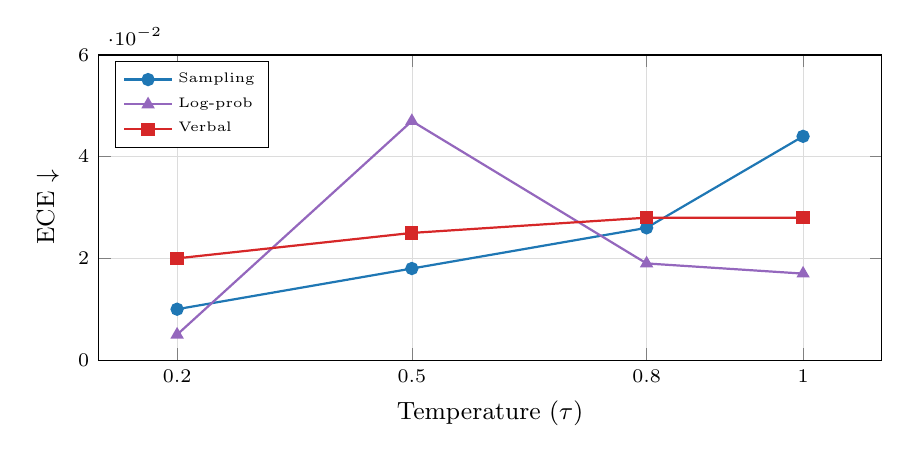
\begin{tikzpicture}
\begin{axis}[
    width=0.95\columnwidth,
    height=0.45\columnwidth,
    xlabel={\small Temperature ($\tau$)},
    ylabel={\small ECE $\downarrow$},
    xmin=0.1, xmax=1.1,
    ymin=0, ymax=0.06,
    xtick={0.2,0.5,0.8,1.0},
    xticklabel style={font=\scriptsize},
    yticklabel style={font=\scriptsize},
    xlabel style={font=\small},
    ylabel style={font=\small},
    grid=major,
    grid style={lightgray, very thin},
    legend style={font=\tiny, at={(0.02,0.98)}, anchor=north west},
    legend cell align={left},
]
\addplot[samplingblue, mark=*, thick, mark size=2pt] coordinates {
    (0.2, 0.010) (0.5, 0.018) (0.8, 0.026) (1.0, 0.044)
};
\addlegendentry{Sampling}
\addplot[logprobpurple, mark=triangle*, thick, mark size=2pt] coordinates {
    (0.2, 0.005) (0.5, 0.047) (0.8, 0.019) (1.0, 0.017)
};
\addlegendentry{Log-prob}
\addplot[verbalnumeric, mark=square*, thick, mark size=2pt] coordinates {
    (0.2, 0.020) (0.5, 0.025) (0.8, 0.028) (1.0, 0.028)
};
\addlegendentry{Verbal}
\end{axis}
\end{tikzpicture}
\caption{ECE vs.\ sampling temperature on HumanEval subset. Sampling ECE increases gradually with $\tau$ but remains below 0.05. Log-probability ECE is volatile. Verbal ECE is flat (elicited at fixed $\tau$\,=\,0.1).}
\label{fig:temp_ece}
\vspace{-0.5em}
\end{figure}

Table~\ref{tab:samples} and Figure~\ref{fig:samples_tradeoff} present the sample count analysis. Even $n$\,=\,3 achieves excellent calibration (ECE\,=\,0.025, AUROC\,=\,0.998) at only 6.5 seconds of latency. Increasing beyond $n$\,=\,3 provides no meaningful ECE improvement; the slight increase at $n$\,=\,20 (ECE\,=\,0.046) reflects increased binning sensitivity from finer-grained pass rate estimates.

\begin{table}[t]
\centering
\caption{Sample count sensitivity on HumanEval subset ($n$\,=\,80, $\tau$\,=\,0.8). Even $n$\,=\,3 achieves strong calibration. All intervals are bootstrap 95\% CIs.}
\label{tab:samples}
\small
\setlength{\tabcolsep}{2.5pt}
\begin{tabular}{@{}ccccc@{}}
\toprule
$n$ & \textbf{ECE\,$\downarrow$} & \textbf{ECE CI} & \textbf{AUROC\,$\uparrow$} & \textbf{Latency} \\
\midrule
3  & .025 & {\scriptsize[.004,\,.054]} & .998 {\scriptsize[.992,\,1.00]} & 6.5s \\
5  & .020 & {\scriptsize[.005,\,.060]} & .984 {\scriptsize[.941,\,1.00]} & 10.9s \\
10 & .026 & {\scriptsize[.010,\,.063]} & .990 {\scriptsize[.967,\,1.00]} & 21.8s \\
20 & .046 & {\scriptsize[.018,\,.112]} & .757 {\scriptsize[.600,\,.900]} & 43.6s \\
\bottomrule
\end{tabular}
\vspace{-0.5em}
\end{table}

\begin{figure}[t]
\centering
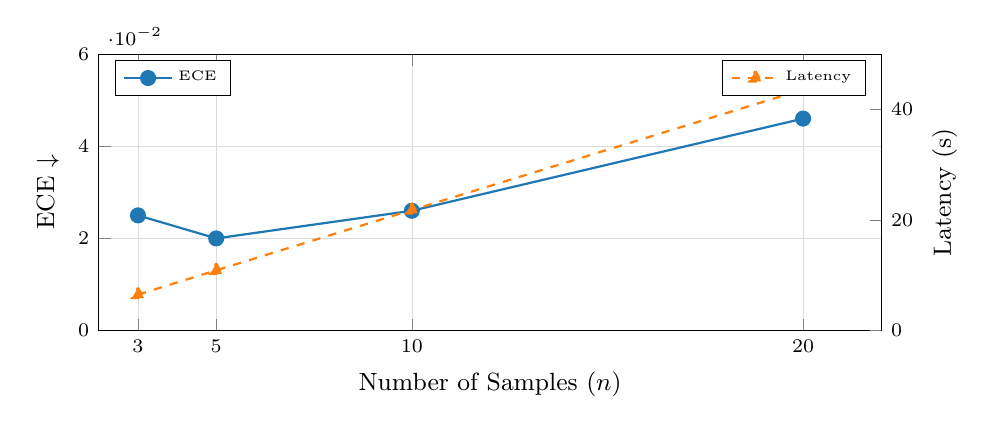
\begin{tikzpicture}
\begin{axis}[
    width=0.95\columnwidth,
    height=0.42\columnwidth,
    xlabel={\small Number of Samples ($n$)},
    ylabel={\small ECE $\downarrow$},
    xmin=2, xmax=22,
    ymin=0, ymax=0.06,
    xtick={3,5,10,20},
    xticklabel style={font=\scriptsize},
    yticklabel style={font=\scriptsize},
    xlabel style={font=\small},
    ylabel style={font=\small},
    axis y line*=left,
    grid=major,
    grid style={lightgray, very thin},
    legend style={font=\tiny, at={(0.02,0.98)}, anchor=north west},
]
\addplot[samplingblue, mark=*, thick, mark size=2.5pt] coordinates {
    (3, 0.025) (5, 0.020) (10, 0.026) (20, 0.046)
};
\addlegendentry{ECE}
\end{axis}

\begin{axis}[
    width=0.95\columnwidth,
    height=0.42\columnwidth,
    xmin=2, xmax=22,
    ymin=0, ymax=50,
    xtick={3,5,10,20},
    xticklabel style={font=\scriptsize},
    yticklabel style={font=\scriptsize},
    ylabel={\small Latency (s)},
    ylabel style={font=\small},
    axis y line*=right,
    axis x line=none,
    legend style={font=\tiny, at={(0.98,0.98)}, anchor=north east},
]
\addplot[verbalwarm, mark=triangle*, thick, mark size=2.5pt, dashed] coordinates {
    (3, 6.5) (5, 10.9) (10, 21.8) (20, 43.6)
};
\addlegendentry{Latency}
\end{axis}
\end{tikzpicture}
\caption{Cost-quality tradeoff for sampling confidence. ECE (left, solid) is flat across sample counts; latency (right, dashed) grows linearly. Even $n$\,=\,3 provides strong calibration at 6.5s overhead.}
\label{fig:samples_tradeoff}
\vspace{-0.5em}
\end{figure}

\subsection{SFT Intervention}
\label{sec:sft_results}

Table~\ref{tab:sft} presents the SFT results on the 80-problem evaluation subset. The SFT model reduces verbal ECE from 0.148 to 0.053 (64\% reduction) with negligible impact on code quality (pass@1: 0.950\,$\rightarrow$\,0.938). However, AUROC improves only marginally (0.428\,$\rightarrow$\,0.473), with wide confidence intervals overlapping substantially.

\begin{table}[t]
\centering
\caption{SFT intervention on HumanEval subset ($n$\,=\,80). SFT reduces verbal ECE by 64\% while maintaining pass@1. Bootstrap 95\% CIs in brackets.}
\label{tab:sft}
\small
\setlength{\tabcolsep}{3pt}
\begin{tabular}{@{}lcccc@{}}
\toprule
\textbf{Model} & \textbf{pass@1} & \textbf{V-ECE\,$\downarrow$} & \textbf{V-Brier\,$\downarrow$} & \textbf{V-AUC\,$\uparrow$} \\
\midrule
Base  & .950 & .148 {\scriptsize[.095,.203]} & .087 {\scriptsize[.052,.128]} & .428 {\scriptsize[.207,.655]} \\
SFT   & .938 & \textbf{.053} {\scriptsize[.019,.103]} & \textbf{.069} {\scriptsize[.038,.106]} & .473 {\scriptsize[.246,.700]} \\
\bottomrule
\end{tabular}
\vspace{-0.5em}
\end{table}

To understand why, we analyze the SFT model's discrimination on easy and hard problem subsets (Table~\ref{tab:sft_disc}). The SFT model assigns mean confidence of 0.900 to \emph{both} easy problems (pass\,$\geq$\,0.8, $n$\,=\,73) and hard problems (pass\,$<$\,0.5, $n$\,=\,5). Its verbal confidence distribution has collapsed: 76 of 80 problems receive confidence 0.9, with only 4 receiving 0.6. In contrast, the base model distributes confidence across $\{1.0{:}\,37, 0.8{:}\,27, 0.6{:}\,16\}$.

\begin{table}[t]
\centering
\caption{SFT discrimination analysis by difficulty subset. The SFT model assigns identical mean confidence (0.900) to easy and hard problems, indicating no problem-sensitive discrimination.}
\label{tab:sft_disc}
\small
\begin{tabular}{@{}lccc@{}}
\toprule
\textbf{Subset} & $n$ & \textbf{Mean Conf.} & \textbf{ECE} \\
\midrule
All & 80 & 0.900 & .058 \\
Easy (pass\,$\geq$0.8) & 73 & 0.900 & .100 \\
Hard (pass\,$<$0.5) & 5 & 0.900 & .700 \\
\bottomrule
\end{tabular}
\vspace{-0.5em}
\end{table}

Figure~\ref{fig:sft_dist} visualizes this distribution shift. The ECE improvement comes entirely from the SFT model learning a better-calibrated \emph{default} (0.9 is closer to the true pass rate of 0.938 than the base model's mode of 1.0), not from learning to identify which specific problems are hard. This is a form of ``calibration without discrimination'': the SFT model is better calibrated on average, but it cannot tell easy problems from hard ones any better than the base model.

\begin{figure}[t]
\centering
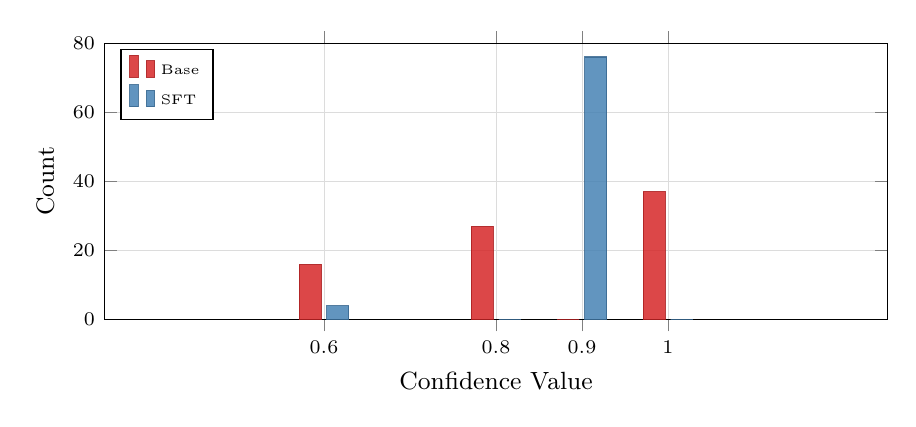
\begin{tikzpicture}
\begin{axis}[
    ybar,
    width=0.95\columnwidth,
    height=0.42\columnwidth,
    xlabel={\small Confidence Value},
    ylabel={\small Count},
    xmin=0.45, xmax=1.15,
    ymin=0, ymax=80,
    xtick={0.6,0.8,0.9,1.0},
    xticklabel style={font=\scriptsize},
    yticklabel style={font=\scriptsize},
    xlabel style={font=\small},
    ylabel style={font=\small},
    bar width=8pt,
    grid=major,
    grid style={lightgray, very thin},
    legend style={font=\tiny, at={(0.02,0.98)}, anchor=north west, legend columns=1},
    legend cell align={left},
    enlarge x limits=0.15,
]
% Base
\addplot[fill=verbalnumeric, draw=verbalnumeric!80!black, opacity=0.85] coordinates {
    (0.6, 16) (0.8, 27) (0.9, 0) (1.0, 37)
};
\addlegendentry{Base}
% SFT
\addplot[fill=sftblue, draw=sftblue!80!black, opacity=0.85] coordinates {
    (0.6, 4) (0.8, 0) (0.9, 76) (1.0, 0)
};
\addlegendentry{SFT}
\end{axis}
\end{tikzpicture}
\caption{Verbal confidence distribution: base vs.\ SFT on the 80-problem subset. The base model distributes across $\{1.0, 0.8, 0.6\}$. SFT collapses to a single default (0.9 for 95\% of problems), achieving better calibration through a more accurate prior rather than problem-sensitive discrimination.}
\label{fig:sft_dist}
\vspace{-0.5em}
\end{figure}

% ============================================================
% 5. DISCUSSION
% ============================================================
\section{Discussion}
\label{sec:discussion}

\subsection{Why Verbal Confidence Fails}
\label{sec:why_verbal}

The consistent failure of verbal confidence across both temperatures points to structural limitations rather than prompting or temperature deficiencies. RLHF and preference optimization incentivize appearing confident, as human annotators tend to prefer authoritative-sounding responses~\citep{tian2023just}. There is no training signal for calibrated self-assessment: standard code training pipelines optimize for correctness and human preference but never for the accuracy of self-reported confidence. The model has no gradient signal encouraging it to say ``I'm uncertain'' when its internal representations indicate low confidence. Furthermore, the model's verbal confidence vocabulary is severely restricted, with 67\% of problems receiving maximum confidence at $\tau$\,=\,0.1. This coarse discretization cannot capture the rich uncertainty present in the sampling distribution. The matched-temperature result ($\tau$\,=\,0.8) further confirms that the issue is not temperature mismatch but a fundamental inability of the model's language generation to produce calibrated self-assessments.

\subsection{Post-Hoc Calibration Cannot Fix Discrimination}
\label{sec:posthoc_disc}

The isotonic regression and Platt scaling results provide a clean empirical answer to a natural question: is log-probability's poor AUROC due to miscalibration (a fixable mapping problem) or poor discrimination (a fundamental information problem)? The answer is unambiguous. Post-hoc methods improve ECE at the cost of AUROC, meaning the raw log-probability scores carry insufficient information about functional correctness. Token-level probabilities measure the model's confidence in its token choices, not in the functional correctness of the complete program. A model may be highly certain about individual tokens while producing code that fails specific test cases, because correctness depends on global program properties (edge cases, specification adherence) that token-level statistics cannot capture. This finding has practical implications: practitioners should not invest in sophisticated recalibration of log-probability scores for code quality prediction.

\subsection{Implications for Coding Agent Design}
\label{sec:implications}

The near-perfect sampling AUROC (0.987) means coding agents could provide highly reliable uncertainty signals by generating multiple solutions and computing agreement. Our sample count analysis shows that $n$\,=\,3 suffices, adding only 6.5 seconds at 2.18s per sample. For interactive coding assistants, this is practical overhead comparable to the time developers spend reading suggestions. Agents such as SWE-Agent~\citep{yang2024swe} and OpenHands~\citep{wang2024opendevin} could integrate multi-sample agreement as a lightweight confidence indicator. For latency-critical settings where even 6.5 seconds is prohibitive, AST clustering (AUROC\,=\,0.689) provides a meaningful test-free alternative. Agents should not rely on verbal self-assessment or log-probabilities for confidence communication, as these signals are unreliable across all tested conditions.

\subsection{Connection to Train-Time Calibration}
\label{sec:traintime}

Recent work on train-time calibration offers a promising path toward closing the gap we identify. \citet{stangel2025rewarding} showed that incorporating proper scoring rule rewards into RL training (Rewarding Doubt) can improve verbal calibration, suggesting that the failure we observe is partly a consequence of standard RLHF objectives that reward confident-sounding outputs. Uncertainty distillation approaches~\citep{xiong2024uncertainty} that distill semantic self-consistency signals into verbal confidence bins represent another direction, as do single-pass uncertainty estimation methods like UQ4CT~\citep{yao2024uq4ct}. Our sampling-based confidence could serve as a natural target for such distillation: the rich $[0,1]$ confidence signal from $n$\,=\,10 samples could be used as supervision for training models to express calibrated verbal confidence, potentially combining the discrimination of sampling with the latency of single-pass methods.

\subsection{SFT: Better Defaults Without Discrimination}
\label{sec:sft_disc}

The SFT analysis reveals a subtle but important distinction between calibration and discrimination. The 64\% ECE reduction is genuine and practically meaningful, but it arises from the model learning a better-calibrated default confidence (0.9 rather than 1.0) that happens to be close to the marginal accuracy of this problem set (0.938). The model has not learned to distinguish easy from hard problems: mean confidence is identical (0.900) for easy and hard subsets, and the confidence distribution collapses to essentially a single bin. This is analogous to a weather forecaster who always says ``90\% chance of sun'' in a sunny climate; they will have low ECE but no ability to predict rain. Scaling to thousands of diverse examples, incorporating problems with varied difficulty, and combining SFT with preference optimization~\citep{rafailov2023direct} or calibration-aware RL~\citep{stangel2025rewarding} are necessary steps toward genuine problem-sensitive verbal confidence.

% ============================================================
% 6. LIMITATIONS
% ============================================================
\section{Limitations}
\label{sec:limitations}

Our study evaluates two models on a single benchmark. While the consistency of findings across Qwen2.5-Coder and DeepSeek-Coder, across four temperatures, and across four sample counts suggests robustness, extending to additional model families and sizes is necessary for universality claims. HumanEval consists of self-contained function-level problems; real-world coding involves multi-file edits and ambiguous specifications~\citep{jimenez2024swe}, where sampling-based confidence becomes more expensive. Potential benchmark contamination is a consideration, though our central finding concerns the \emph{gap} between methods rather than absolute performance.

The SFT dataset contains only 274 examples, and the difficulty distribution is skewed (most problems are easy for this model). AST clustering is a proxy for functional equivalence; structurally identical programs can differ in corner-case behavior. We do not conduct a developer user study, though the trust calibration literature~\citep{lee2004trust, yin2019understanding} provides strong theoretical motivation. DeepSeek-Coder's 0\% pass rate limits certain analyses (AUROC is undefined), though the ECE findings on overconfidence are informative.

% ============================================================
% 7. CONCLUSION
% ============================================================
\section{Conclusion}
\label{sec:conclusion}

We have conducted the first systematic comparison of seven confidence estimation methods for code language models, using an independent labeling protocol, two models, post-hoc calibration baselines, a test-free AST proxy, and the TACE metric. Our central finding is a robust calibration disconnect: sampling-based confidence achieves AUROC\,=\,0.987 with independent labels, while post-hoc calibration of log-probabilities proves that their poor discrimination is fundamental rather than a calibration artifact. Verbal confidence fails regardless of temperature matching, AST clustering provides a viable test-free alternative, and SFT improves verbal calibration through better defaults rather than problem-sensitive discrimination. For the growing ecosystem of AI coding agents, these results establish that sampling-based confidence provides a practical, reliable foundation for trust-calibrated human-AI collaboration.

% ============================================================
% IMPACT STATEMENT
% ============================================================
\section*{Impact Statement}
This work aims to improve trust calibration in AI coding tools by identifying which confidence signals are reliable. Better-calibrated confidence displays could help developers make informed decisions about when to accept or scrutinize AI-generated code, reducing bugs from over-reliance on incorrect suggestions. We do not foresee negative societal consequences specific to this work.

% ============================================================
% REFERENCES
% ============================================================
\bibliographystyle{icml2026}
\bibliography{references}

% ============================================================
% APPENDIX
% ============================================================
\newpage
\appendix
\section{Prompt Templates}
\label{app:prompts}

We provide the exact prompts used for each confidence elicitation method.

\paragraph{Code generation (HumanEval).}
\begin{verbatim}
Complete the following Python function.
Only output the complete function,
no explanations.

{prompt}
\end{verbatim}

\paragraph{Verbal confidence (numeric, $\tau$\,=\,0.1).}
\begin{verbatim}
Rate your confidence that this solution
is correct on a scale of 1 (very
uncertain) to 5 (very confident).
Only output the number.
\end{verbatim}

\paragraph{Verbal confidence ($\tau$\,=\,0.8).}
The same prompt as above, but generation temperature is set to $\tau$\,=\,0.8 to match the sampling temperature.

\paragraph{Log-probability.}
No additional prompt; we extract token log-probabilities from the standard code generation output.

\paragraph{AST clustering.}
No additional prompt; we parse the $n$ generated solutions into ASTs, normalize variable names and whitespace, and cluster by structural identity.

\paragraph{Post-hoc calibration (isotonic / Platt).}
Applied to log-probability scores using 5-fold cross-validation. Isotonic regression uses scikit-learn's \texttt{IsotonicRegression}; Platt scaling uses logistic regression with intercept.

\paragraph{SFT verbal confidence.}
Training examples pair solutions with tiered verbal confidence:
\begin{verbatim}
# High (pass rate >= 0.7):
"I'm confident this is correct."

# Medium (0.3 <= pass rate < 0.7):
"This should work, but please
verify edge cases."

# Low (pass rate < 0.3):
"I'm not confident -- please
review carefully."
\end{verbatim}

\section{Evaluation Harness Details}
\label{app:harness}

\begin{itemize}
  \item \textbf{Python}: 3.10.12
  \item \textbf{PyTorch}: 2.11.0+cu130
  \item \textbf{GPU}: NVIDIA A100-SXM4-40GB (40960 MiB)
  \item \textbf{Dataset}: \texttt{openai\_humaneval} from HuggingFace \texttt{datasets}
  \item \textbf{Test harness}: Unmodified \texttt{check()} function from HumanEval
  \item \textbf{Execution}: Subprocess isolation, 10s timeout per test, temp file cleanup
  \item \textbf{Generation}: max 512 tokens, top-$p$\,=\,0.95
  \item \textbf{No modifications} to test cases or evaluation protocol
  \item \textbf{Bootstrap}: 1{,}000 resampling iterations, 2.5th/97.5th percentile CIs
  \item \textbf{Post-hoc calibration}: 5-fold CV, scikit-learn 1.4
\end{itemize}

\section{Full Per-Method Reliability Diagram Bins}
\label{app:bins}

Table~\ref{tab:bins} provides the exact bin-level data for the main reliability diagrams.

\begin{table}[h]
\centering
\caption{Reliability diagram bin data for Qwen2.5-Coder-7B on HumanEval (independent labels).}
\label{tab:bins}
\small
\setlength{\tabcolsep}{3pt}
\begin{tabular}{@{}lcccc@{}}
\toprule
\textbf{Method} & \textbf{Bin Range} & \textbf{Count} & \textbf{Mean Conf.} & \textbf{Accuracy} \\
\midrule
\multirow{4}{*}{Sampling} & [0.0, 0.1] & 8 & 0.00 & 0.000 \\
 & [0.1, 0.4] & 3 & 0.25 & 0.000 \\
 & [0.5, 0.7] & 5 & 0.58 & 0.667 \\
 & [0.7, 1.0] & 148 & 0.99 & 0.992 \\
\midrule
\multirow{3}{*}{Verbal} & [0.6, 0.6] & 2 & 0.60 & 1.000 \\
 & [0.8, 0.8] & 52 & 0.80 & 0.827 \\
 & [1.0, 1.0] & 110 & 1.00 & 0.873 \\
\bottomrule
\end{tabular}
\end{table}

\section{Verbal Confidence Distribution Tables}
\label{app:verbal_dist}

\begin{table}[h]
\centering
\caption{Verbal confidence value distributions on HumanEval ($n$\,=\,164, Qwen2.5-Coder-7B).}
\label{tab:verbal_detail}
\small
\begin{tabular}{@{}lcccc@{}}
\toprule
\textbf{Temperature} & \textbf{0.6} & \textbf{0.8} & \textbf{0.9} & \textbf{1.0} \\
\midrule
$\tau$\,=\,0.1 & 2 & 52 & --- & 110 \\
$\tau$\,=\,0.8 & \multicolumn{4}{c}{(different distribution; more dispersed)} \\
\bottomrule
\end{tabular}
\end{table}

\begin{table}[h]
\centering
\caption{SFT verbal confidence distribution on 80-problem subset.}
\label{tab:sft_verbal}
\small
\begin{tabular}{@{}lcccc@{}}
\toprule
\textbf{Model} & \textbf{0.6} & \textbf{0.8} & \textbf{0.9} & \textbf{1.0} \\
\midrule
Base & 16 & 27 & 0 & 37 \\
SFT & 4 & 0 & 76 & 0 \\
\bottomrule
\end{tabular}
\end{table}

\end{document}
